\documentclass{article}
\usepackage{graphicx}
\usepackage{amssymb}
\usepackage{amsmath}
\usepackage{float}
\usepackage{hyperref}
\usepackage{algorithm2e}
\usepackage[margin=1in]{geometry}

\begin{document}

\title{Robotics 811 - Homework 4}
\author{Xiang Zhi Tan}
\maketitle

\section{Q1}
\subsection*{1(a)}
Fristly, we notice that the equation is a separative form of differentiation and can be separate into 
\begin{equation*}
\begin{aligned}
\frac{dy}{dx} &= \frac{2}{x^2} (1-y) \\
(1-y) dy &= \frac{2}{x^2} dx 
\end{aligned}
\end{equation*}
By applying integration to both side, we get
\begin{equation*}
\begin{aligned}
\int (1-y) dy &= \int \frac{2}{x^2} dx \\
y - \frac{1}{2}y^2 + c &= -2 x^{-1} + c
\end{aligned}
\end{equation*}
By observing the equation, we notice it has the form of a quadratic equation, we then rearrange it and put it into the form of the quadratic formula.
\begin{equation*}
\begin{aligned}
y - \frac{1}{2}y^2 + c &= -2 x^{-1} + c\\
-\frac{1}{2}y^2 + y +(2x^{-1} - c) &= 0\\
y^2 + (-2y) +(-4x^{-1} + c) &= 0\\
y &= \frac{2 \pm \sqrt{4 - 4(-4x^{-1} + c)}}{2}\\
y &= 1 \pm \frac{\sqrt{4 + 16x^{-1} - 4c}}{2}\\
y &= 1 \pm \frac{\sqrt{4}\sqrt{1 + 4x^{-1} - c}}{2}\\
y &= 1 \pm \sqrt{1 + 4x^{-1} -c}\\
y &= 1 \pm \sqrt{4x^{-1} - c}
\end{aligned}
\end{equation*}
Because we know the initial condition of $y(1) = -1$, we can plug it back into the previous equation and solve for $c$
\begin{equation*}
-1 = 1 \pm \sqrt{\frac{4}{1} - c}
\end{equation*}
Because the square root will be positive, the only way to have a negative on the lefthand side would be that the $\pm$ is a negative sign.
\begin{equation*}
\begin{aligned}
-1 &= 1 - \sqrt{4 - c}\\
2 &= \sqrt{4 - c}\\
c & = 0 
\end{aligned}
\end{equation*}
Now, we know that the analytic solution would be the following:
\begin{equation*}
y(x) = 1 - 2 \sqrt{x^{-1}}
\end{equation*}
\subsection*{1(b)}
We implemented the Euler Method in the matlab script, \textbf{q1b.m}. Below is the result of the Method at each $x$ with a step size of $0.05$, x and the real y in table form.
\begin{center}
\begin{tabular}{|c|c|c|c|}
\hline
n & x & y & real y \\ \hline
0 & 1.000000 & -1.000000 & -1.000000 \\ \hline 
1 & 0.950000 & -1.050000 & -1.051957 \\ \hline 
2 & 0.900000 & -1.104050 & -1.108185 \\ \hline 
3 & 0.850000 & -1.162726 & -1.169305 \\ \hline 
4 & 0.800000 & -1.226723 & -1.236068 \\ \hline 
5 & 0.750000 & -1.296894 & -1.309401 \\ \hline 
6 & 0.700000 & -1.374293 & -1.390457 \\ \hline 
7 & 0.650000 & -1.460248 & -1.480695 \\ \hline 
8 & 0.600000 & -1.556452 & -1.581989 \\ \hline 
9 & 0.550000 & -1.665109 & -1.696799 \\ \hline 
10 & 0.500000 & -1.789149 & -1.828427 \\ \hline 
11 & 0.450000 & -1.932562 & -1.981424 \\ \hline 
12 & 0.400000 & -2.100956 & -2.162278 \\ \hline 
13 & 0.350000 & -2.302507 & -2.380617 \\ \hline 
14 & 0.300000 & -2.549691 & -2.651484 \\ \hline 
15 & 0.250000 & -2.862707 & -3.000000 \\ \hline 
16 & 0.200000 & -3.276924 & -3.472136 \\ \hline 
17 & 0.150000 & -3.861457 & -4.163978 \\ \hline 
18 & 0.100000 & -4.775677 & -5.324555 \\ \hline 
19 & 0.050000 & -6.507076 & -7.944272 \\ \hline 
20 & 0.000000 & -11.835382 & -Inf \\ \hline 
\end{tabular}
\end{center}
By observing the values, we notice this method is not too accurate and there are deviation in the end values.
\begin{equation*}
\end{equation*}
\subsection*{1(c)}
We implemented the fourth-order Runge-Kutta method in the matlab script, \textbf{q1c.m}. Below is the result of the Method at each $x$ with a step size of $0.05$, x and the real y in table form.
\begin{center}
\begin{tabular}{|c|c|c|c|}
\hline
n & x & y & real y \\ \hline
0 & 1.000000 & -1.000000 & -1.000000 \\ \hline 
1 & 0.950000 & -1.051957 & -1.051957 \\ \hline 
2 & 0.900000 & -1.108185 & -1.108185 \\ \hline 
3 & 0.850000 & -1.169305 & -1.169305 \\ \hline 
4 & 0.800000 & -1.236068 & -1.236068 \\ \hline 
5 & 0.750000 & -1.309401 & -1.309401 \\ \hline 
6 & 0.700000 & -1.390457 & -1.390457 \\ \hline 
7 & 0.650000 & -1.480695 & -1.480695 \\ \hline 
8 & 0.600000 & -1.581990 & -1.581989 \\ \hline 
9 & 0.550000 & -1.696800 & -1.696799 \\ \hline 
10 & 0.500000 & -1.828429 & -1.828427 \\ \hline 
11 & 0.450000 & -1.981426 & -1.981424 \\ \hline 
12 & 0.400000 & -2.162282 & -2.162278 \\ \hline 
13 & 0.350000 & -2.380624 & -2.380617 \\ \hline 
14 & 0.300000 & -2.651498 & -2.651484 \\ \hline 
15 & 0.250000 & -3.000033 & -3.000000 \\ \hline 
16 & 0.200000 & -3.472225 & -3.472136 \\ \hline 
17 & 0.150000 & -4.164292 & -4.163978 \\ \hline 
18 & 0.100000 & -5.326343 & -5.324555 \\ \hline 
19 & 0.050000 & -7.973392 & -7.944272 \\ \hline 
20 & 0.000000 & -183129202253624666683263156224.000000 & -Inf \\ \hline 
\end{tabular}
\end{center}
By observing the result, we observe that the values don't deviate until $n=8$. Compared to Euler methods, fourth-order Runge-Kutta method is more accurate.
\subsection*{1(d)}
We implemented the fourth-order Adams-Bashforth in the script, \textbf{q1d.m}. Below is the result of the Method at each $x$ with a step size of $0.05$, x and the real y in table form. Compared to the analytic solution, the results deviates faster as x approaches 0. 
\begin{center}
\begin{tabular}{|c|c|c|c|}
\hline
0 & 1.000000 & -1.000000 & -1.000000 \\ \hline 
1 & 0.950000 & -1.051952 & -1.051957 \\ \hline 
2 & 0.900000 & -1.108174 & -1.108185 \\ \hline 
3 & 0.850000 & -1.169285 & -1.169305 \\ \hline 
4 & 0.800000 & -1.236038 & -1.236068 \\ \hline 
5 & 0.750000 & -1.309357 & -1.309401 \\ \hline 
6 & 0.700000 & -1.390393 & -1.390457 \\ \hline 
7 & 0.650000 & -1.480601 & -1.480695 \\ \hline 
8 & 0.600000 & -1.581854 & -1.581989 \\ \hline 
9 & 0.550000 & -1.696602 & -1.696799 \\ \hline 
10 & 0.500000 & -1.828133 & -1.828427 \\ \hline 
11 & 0.450000 & -1.980974 & -1.981424 \\ \hline 
12 & 0.400000 & -2.161562 & -2.162278 \\ \hline 
13 & 0.350000 & -2.379424 & -2.380617 \\ \hline 
14 & 0.300000 & -2.649367 & -2.651484 \\ \hline 
15 & 0.250000 & -2.995918 & -3.000000 \\ \hline 
16 & 0.200000 & -3.463310 & -3.472136 \\ \hline 
17 & 0.150000 & -4.141388 & -4.163978 \\ \hline 
18 & 0.100000 & -5.248560 & -5.324555 \\ \hline 
19 & 0.050000 & -7.504348 & -7.944272 \\ \hline 
20 & 0.000000 & -15.471548 & -Inf \\ \hline 
\end{tabular}
\end{center}
By observing the result, we see that the fourth-order Adams-Bashforth is more accurate than Euler's method but less accurate then fourth-order Runge-Kutta method.
\section{Q2}

\subsection*{2(a)}
Firstly, we plotted the function in matlab using the \textit{contour} function on the range, $y=[-4,2]$ and $x=[-2,4]$. Following is the result of the contour plot
\begin{figure}[H]
\centering
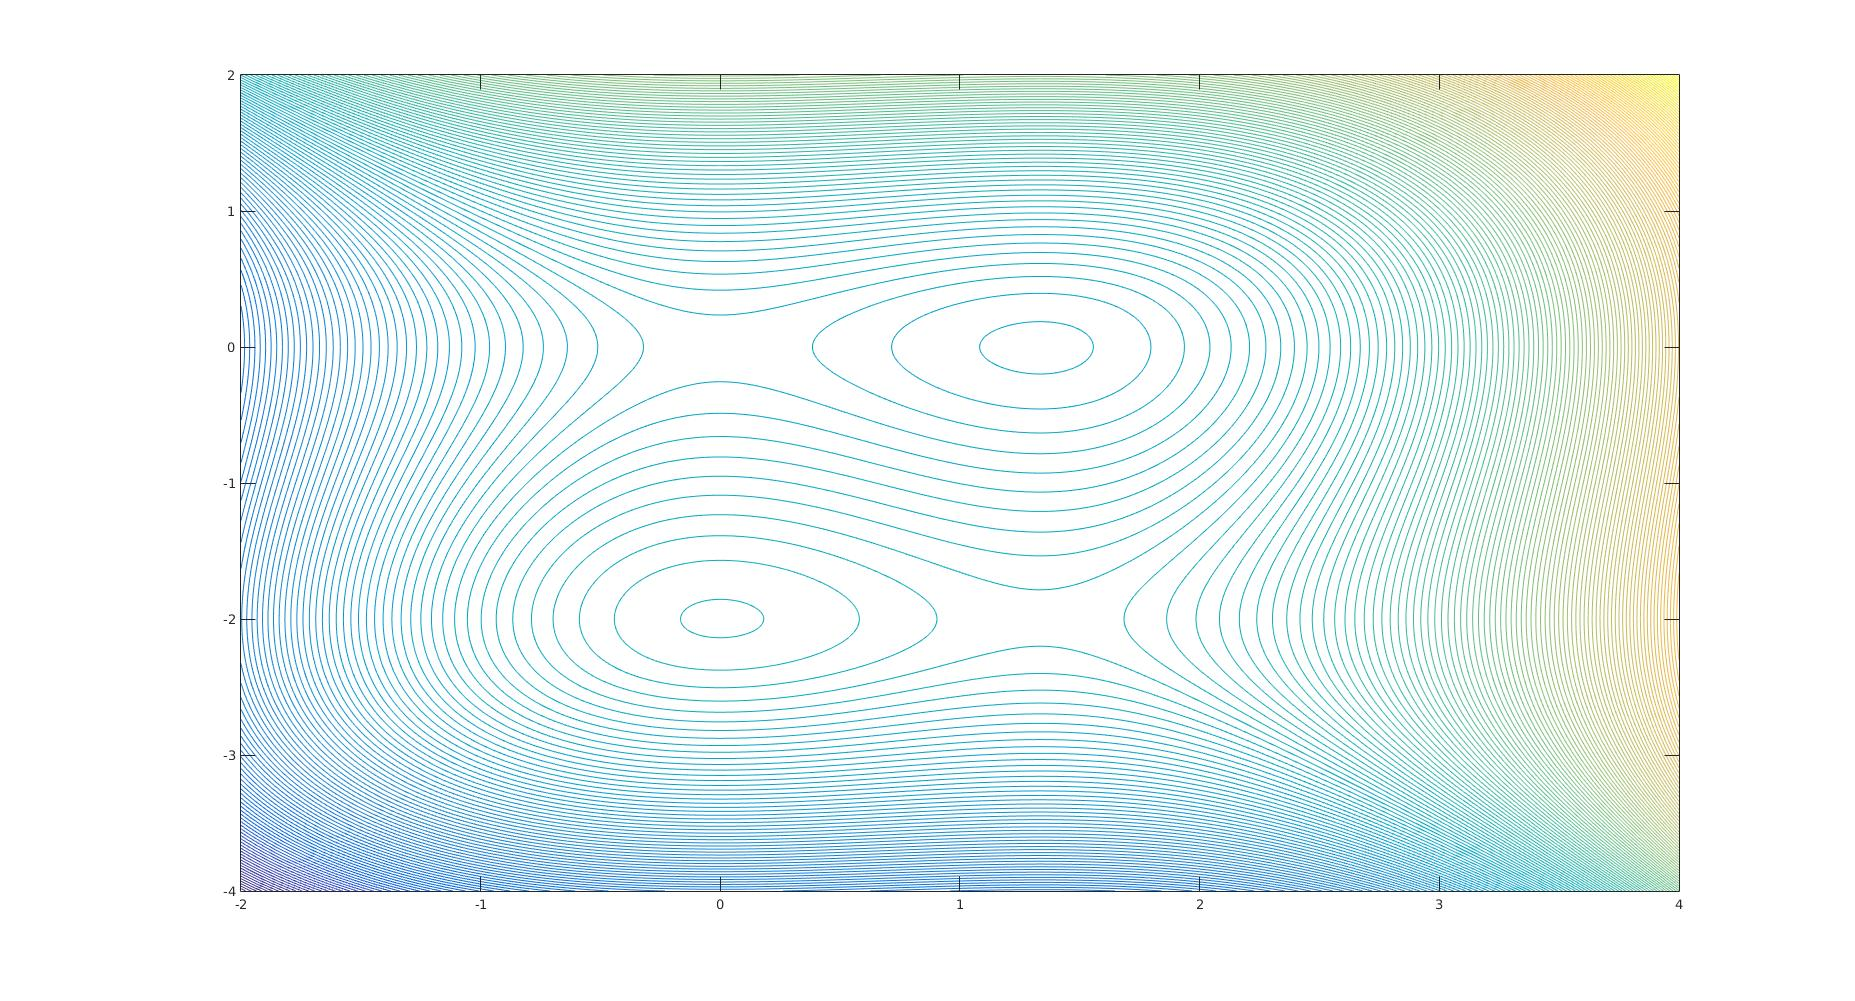
\includegraphics[width=6.5in]{figures/2a.jpg}
\caption{plot of the function $f(x,y) = x^3 + y^3 -2x^2 + 3y^2 - 8$}
\end{figure}
By examining the sketch created, we notice there are four critical points, $(0,-2),(0,0),(\frac{4}{3},-2),(\frac{4}{3},0)$.
We then measure the gradients(in the domain space) of the nearby points to determine the type of critical point. 
Following are the finding for each point:
\begin{enumerate}
\item Point$(0,-2)$\\
This is a local maxima. By measuring the gradient at 8 points around the point with a step size of $0.1$ relative to this point. we found them all to have a position gradient which means they are moving upwards towards $(0,-2)$ which means this is a local maximum.
\item Point$(0,0)$\\
This is a saddle points. When measuring the gradient at 8 points around the point with a step size of $0.1$ relative to this point, we measured a positive gradient at the two points of $(0.1,0)$ and $(-0.1,0)$ and the remaining 6 points to have a negative gradient. This fits the definition of a saddle point.
\item Point$(\frac{4}{3},0)$\\
This is the local minima. When measuring the gradient at the 8 points around the point with the step size of $0.1$ relative to this point, all gradients are negative, this means that the direction of all these points are towards this point, meaning that this point must serve as the local minima.
\item Point$(\frac{4}{3},-2)$\\
This is a saddle points. When measuring the gradient, we found a negative gradient at points $(1.23333,-2)$ and $(1.43333,-2)$ and positive gradient at all remaining points. This shows that this must be a saddle point.
\subsection*{2(b)}
The gradient(partial derivative) of x and y can be found with the following equation:
\begin{equation*}
\begin{aligned}
\frac{\partial}{\partial x}  = x(3x - 4)\\
\frac{\partial}{\partial y}  = y(3y + 6)
\end{aligned}
\end{equation*}
Using the steepest descent algorithm, we first calculate the gradient at point $(1,-1)$. Which gives us the gradient at x, $\frac{\partial}{\partial x} = -1$ and gradient at y, $\frac{\partial}{\partial y} = -3$. Since the gradient are both non zero, we try to minimize the function $g(t) = f(x + t\vec{u})$ with u being the gradient. Minimizing the function, we found $t = \frac{1}{3}$. We update the points using the following algorithm $x^{n+1} = x^{n} - t\vec{u}$. After updating the points, we found the points to be $(\frac{4}{3},0)$ which is one of the critical points(also the local minima). The gradient at that point is also $0$, stopping the algorithm. Therefore, we need only one step to converge to the local minimum, if we start steepest descent at point $(1,-1)$.

\end{enumerate}
\section{Q3}
\subsection*{3(a)}
First, we know that eigenvectors of Q(real symmetric positive definite matrix) are orthogonal(proof of this could be easily found online or derived). This means that given two eigenvectors, $v_1$ and $v_2$ come from two distinct eigenvalues, $\lambda_1$ and $\lambda_2$, their inner product would be 0. By grinding through the equations, we could derive the Q-orthogonal definition.
\begin{equation*}
\begin{aligned}
<v_1, v_2> &= 0&\\
<\lambda_1 v_1, v2> &= 0  &\mbox{  $\lambda$ is a scalar and will not change the result of the inner product}\\
<Q v_1, v_2> &= 0 &\\
(Q v_1)^Tv_2 &= 0 &\\
v_1^T Q^Tv_2 &= 0& \mbox{ $Q^T=Q$}\\
v_1^T Q v_2 &= 0 &\mbox{   the definition of Q-orthogonal}
\end{aligned}
\end{equation*}
\subsection*{3(b)}
The solution in the previous section would be sufficient as it is based on the fact that eigenvectors of Q are orthogonal to each other, which is now explicitly given.
\section{Q4}
I discussed with Rick Goldstein on parts of the problem
\subsection*{4(a)}
From the algorithm in the notes on page 17, we know that:
\begin{equation} \label{4-e1}
d_k = -g_k + B_{k-1}d_{k-1}
\end{equation}
As we want to show $d_k^TQd_k = -d_k^TQg_k$, we will derive the right-hand side from the left using equation \ref{4-e1}.
\begin{equation}\label{4-e2}
\begin{aligned}
d_k^TQd_k &= d_k^TQ(-g_k + B_{k-1}d_{k-1}) &\mbox{ ,inserted \ref{4-e1}}\\
&= -d_k^TQg_k +  B_{k-1}d_k^TQd_{k-1} &\mbox{ , $d_k$ and $d_{k-1}$ are Q-orthogonal, $d_k^TQd_{k-1}=0$} \\
&= -d_k^TQg_k
\end{aligned}
\end{equation}
This shows that $d_k^TQd_k = -d_k^TQg_k$. Now we will show that we can obtain $x_{k+1}$ with only $Q$ to find $g_k$ and $Qg_k$.
First is obtaining $d_k$.
\begin{equation}\label{4-e21}
\begin{aligned}
d_k &= - g_k + B_{k-1}d_{k-1}&\\
& = - g_k + \frac{g_k^TQd_{k-1}}{d_{k-1}^TQd_{k-1}} d_{k-1}&\\
& = - g_k - \frac{d_{k-1}^TQg_k}{d_{k-1}^TQg_{k-1}} d_{k-1}& \mbox{, rearrange and apply \ref{4-e2}}
\end{aligned}
\end{equation}
Obtaining $d_k$ now only depends on $d_{k-1}$, which is obtain in the previous iterative or given if it's the first, $Qg_{k-1}$ and $g_k$, which is what we want.\\
Now we will see how to obtain $\alpha_k$
\begin{equation}\label{4-e22}
\begin{aligned}
\alpha_k &= - \frac{g_k^Td_k}{d_k^TQd_k}&\\
\alpha_k &= \frac{g_k^Td_k}{d_k^TQg_k}& \mbox{, apply \ref{4-e2}}\\
\end{aligned}
\end{equation}
Again, obtaining $\alpha_k$ would only need variables that we already calculated. To get $x_k+1$ would just be $x_{k+1} = x_k + \alpha_k d_k$. Which both have been shown to be able to be derived using only $Q$ to evaluate $g_k$ and $Qg_k$.
\subsection*{4(b)}
We will derive the desire solution using the fact that $y_k = x_k - g_k$ and $p_k = \Delta f(y_k)$.
\begin{equation}\label{4-e3}
\begin{aligned}
p_k &= \Delta f(y_k) &\\
&= Q(y_k) + b & \mbox{wrote the gradient in terms of equation}\\
&= Q(x_k - g_k) + b &\\
&= Qx_k - Qg_k + b &\\
&= Qx_k + b - Qg_k&\\
&= g_k - Qg_k & \mbox{ , $Qx_k + b$ is the gradient at the point $x_k$, therefore can be written as $g_k$}\\
Qg_k &= g_k - p_k &\\ 
\end{aligned}
\end{equation}

\subsection*{4(c)}
First, we will modified some terms in the original algorithm in the notes on page 17 using the equations \ref{4-e2} and \ref{4-e3}.\\
For equation 2(a) in the notes which has already been modified in \ref{4-e22}
\begin{equation*}
\begin{aligned}
\alpha_k &= \frac{g_k^Td_k}{d_k^TQg_k}\\
\alpha_k &= \frac{g_k^Td_k}{d_k^T(g_k - p_k)} \mbox{ ,applied \ref{4-e3}}
\end{aligned}
\end{equation*}
For equation 2(c) in the notes.
\begin{equation}
\begin{aligned}
B_k &= \frac{g_{k+1}^TQd_k}{d_k^TQg_k}&\\
&= \frac{d_{k}^TQg_{k+1}}{d_{k}^TQg_{k}}&\\
&= \frac{d_k(g_{k+1} - p_{k+1})}{d_k^T(g_k - p_k)}& \mbox{ ,applied \ref{4-e3}}
\end{aligned}
\end{equation}

The final general algorithm will be similar to the one in the notes on page 17.\\
\begin{algorithm}[H]
  \KwResult{Minimum of the equation}
  Let $d_0$ = $-g_0$\;
  \For{$k = 0,...,n-1$}{
  	$\alpha_k = \frac{g_k^Td_k}{d_k^T(g_k - p_k)}$\;
  	$x_{k+1} = x_k + \alpha_k d_k$\;
  	$B_k = \frac{d_k(g_{k+1} - p_{k+1})}{d_k^T(g_k - p_k)}$\;
  	$d_{k+1} = - g_{k+1} + B_k d_k$
  }
  Return $X_n$\;
  \caption{Conjugate Gradient Method}
\end{algorithm}
Note, the gradient of each point can be obtain by sampling the surrounding points
\section{Q5}
The order of the direction searched does not matter. This is because $Q$ is a symmetric positive definite matrix and this makes the $d_0,d_1,...,d_k$ vectors Q-orthogonal and linearly independent(proof on page 14 of notes).This mean each individual $d$ are independent and does not depend on prior directions. As $k$ increases in the search, it will slowly search a larger spam subspace and in the end find the minimum of the whole function space at $k=n-1$. The order doesn't matter as any permutation of the search will eventually give the same result.
Furthermore, we will only need to search each direction onces. This is because of the Expanding subspace theorem(in notes page 20) that states that for all $x$ in the sequence ${x_k}$ generated by the following rule
\begin{equation*}
\begin{aligned}
x_{k+1} &= x_k + \alpha_k d_k\\
\mbox{ where } \alpha_k &= - \frac{g_k^Td_k}{d_k^TQd_k}\\
g_k &= QX_k + b
\end{aligned}
\end{equation*}
The generated $x_{k+1}$ will be the minimum of the line $x_{k+1} + \alpha_k d_k$. This means that at one search along the line, it will find the minimum in that space. Furthermore, the Expanding subspace theorem also minimizes on the affine variety, $x_0 + B_{k+1}$. The $x_k+1$ we find is the minimum of the span of all the previous direction($d_0, d_1, ... d_k$) as well, means that there are no other point in that subspace that could be smaller than the found $x_k+1$. Therefore, we will only need to search the direction once for each direction.
\section{Q6}
%question 6

As we are finding the maximum area with a given parameter,$p$, we know that the objective function must be
\begin{equation*}
f(x,y) = xy
\end{equation*}
with the constraint of 
\begin{equation*}
2y + 2x - p = 0
\end{equation*}
First we construct the Lagrangian
\begin{equation*}
L(x,y,\alpha) = xy + \alpha(2y + 2x - p)
\end{equation*}
We then compute the gradient at set it to 0
\begin{equation*}
\Delta L(x,y,\alpha) = 
\begin{pmatrix}
y + 2\alpha\\
x + 2\alpha\\
2x + 2y -p \\
\end{pmatrix}
= \vec{0}
\end{equation*}
We are now given 3 equations
\begin{equation}\label{e1}
y = 2\alpha
\end{equation}
\begin{equation}\label{e2}
x = 2\alpha
\end{equation}
\begin{equation}
\begin{aligned}\label{e3}
2x &= -2y + p \\
x = \frac{-2y + p}{2}
\end{aligned}
\end{equation}
Insert \ref{e3} into \ref{e2}, we get
\begin{equation}\label{e4}
2 \alpha = \frac{-2y + p}{2}
\end{equation}
Then, insert \ref{e4} into \ref{e1}, we can solve $y$
\begin{equation}\label{e5}
\begin{aligned}
y &= \frac{-2y + p}{2}\\
2y &= -2y + p\\
y = \frac{p}{4}
\end{aligned}
\end{equation}
We then insert \ref{e5} back into \ref{e2} and we solve $x$
\begin{equation}
x = \frac{p}{4}
\end{equation}
We have now found the critical points in the equation, where $x = \frac{p}{4}$ and $y=\frac{p}{4}$. Notice that $x = y$. To show that we are achieving the maximum, we need to verify the second order sufficiency where we need to show the following matrix
\begin{equation}
L(x^*) = \Delta^2f(x*) + \alpha^T\Delta^2h(x^*)
\end{equation}
is negative semi-definate on $m$ which is $m = {y | \Delta h (x^*) y = 0}$. First we solve the partial derivatives for $f(x)$ and $h(x)$
\begin{equation*}
\begin{aligned}
\frac{\partial}{\partial^2 x} &= 0\\
\frac{\partial}{\partial^2 y} &= 0\\
\frac{\partial}{\partial xy} &= 1\\
\frac{\partial}{\partial yx} &= 1\\
\Delta^2 h &= 0\\
\end{aligned}
\end{equation*}
We have solved $L(x^*)$
\begin{equation*}
L(x^*) = 
\begin{pmatrix}
0 &1\\
1 &0\\
\end{pmatrix}
\end{equation*}
We then check where the matrix is positive semi-definite or negative semi-definite by choosing a vector from the subspace $M$ and apply $y^TLy$.
\begin{equation}
\begin{aligned}
\Delta h(x) &= [2 2]\\
[2 2]y &= 0\\
\begin{pmatrix}
y_1\\
y_2 \\
\end{pmatrix}
& = 
\begin{pmatrix}
-1 \\
1 \\
\end{pmatrix}
\end{aligned}
\end{equation} 
\begin{equation}
\begin{pmatrix}
-1 & 1 
\end{pmatrix}
\begin{pmatrix}
0 & 1 \\
1 & 0\\
\end{pmatrix}
\begin{pmatrix}
-1 \\
1
\end{pmatrix}
= -2
\end{equation}
This shows the matrix is negative semi-definite and therefore, $x^*$ must be the maximum of $f$.

\section{Q7}
\subsection*{7(a)}
We can first rearrange the constraints 2 and 3 into the following form by moving elements on the right handside to the left and multiplying constraints 2 by $-1$.
\begin{equation*}
\begin{aligned}
- w^Tx_i - b + 1 - \xi_i &\leq 0\\ \mbox{ if } y_i = 1
w^Tx_i + b + 1 - \xi_i &\leq 0\\ \mbox{ if } y_i = -1
\end{aligned} 
\end{equation*}
Through observing the inequalities, we notice that the only difference is the element $w^Tx_i$ which has a different sign that could be change by the values of $y_i$. This allows us to combine both inequalities into the following constraint.
\begin{equation*}
- y_i(w^Tx_i + b) + 1 - \xi_i \leq = 0
\end{equation*}

\subsection*{7(b)}
The Lagrangian for our optimization problem is as following:
\begin{equation*}
L ([w\;0\;\xi]^T, \alpha, \beta) = \frac{1}{2}||w||^2 + C \sum_{i=1}^l \xi_i + \sum_{i=1}^l \alpha_ig_i([w\;b\;\xi]^T) - \sum_{i=1}^l \beta_i \xi_i
\end{equation*}

\subsection*{7(c)}
Following is the steps to minimize the Lagrangian which is ther primal form of the SVM. Here's the original Lagrangian.
\begin{equation}\label{ori-l}
L ([w\;0\;\xi]^T, \alpha, \beta) = \frac{1}{2}||w||^2 + C \sum_{i=1}^l \xi_i + \sum_{i=1}^l \alpha_i(- y_i(w^Tx_i + b) + 1 - \xi_i) - \sum_{i=1}^l \beta_i \xi_i
\end{equation}
First we, find the partial of $w$,$b$ and $\xi_i$. Following are the partials follow by setting them to 0.\\
Finding partial of $w$
\begin{equation}\label{wpartial}
\begin{aligned}
\frac{\partial}{\partial w} &= \frac{2}{2} w - \sum_{i=1}^l(\alpha_i y_i x_i) = 0\\
w &= \sum_{i=1}^l(\alpha_i y_i x_i)
\end{aligned}
\end{equation}
Finding the partial of $b$.
\begin{equation}\label{bpartial}
\begin{aligned}
\frac{\partial}{\partial b} &= -\sum_{i=1}^l(\alpha_i y_i) = 0\\
\sum_{i=1}^l(\alpha_i y_i) &= 0\\
\end{aligned}
\end{equation}
Finding the partial of $xi_i$.
\begin{equation}\label{xipartial}
\begin{aligned}
\frac{\partial}{\partial \xi_i} &= C - \sum_{i=1}^l(\alpha_i) - \sum_{i=1}^l(\beta_i) = 0\\
C &= \sum_{i=1}^l(\alpha_i) + \sum_{i=1}^l(\beta_i)
\end{aligned}
\end{equation}\tabularnewline
Now we insert equations \ref{wpartial}, \ref{xipartial} in equation \ref{ori-l}.
\begin{equation}
\begin{aligned}
L &= \frac{1}{2}(\sum_{i=1}^l(\alpha_i y_i x_i))^2 + (\sum_{i=1}^l(\alpha_i) + \sum_{i=1}^l(\beta_i))\sum_{i=1}^l \xi_i + \sum_{i=1}^l \alpha_i(- y_i((\sum_{j=1}^l(\alpha_j y_j x_j))x_i + b) + 1 - \xi_i) - \sum_{i=1}^l \beta_i \xi_i\\
L &= \frac{1}{2}(\sum_{i=1}^l\sum_{j=1}^l(\alpha_i \alpha_j y_i y_j x_j^T x_i)) + \sum_{i=1}^l(\alpha_i \xi_i) + \sum_{i=1}^l(\beta_i \xi_i) + \sum_{i=1}^l(\alpha_i \alpha_j y_i y_j x_j^T x_i))\\
&- b \sum_{i=1}^l(\alpha_i y_i) + \sum_{i=1}^l(\alpha_i) - \sum_{i=1}^l(\alpha_i \xi_i) - \sum_{i=1}^l \beta_i \xi_i\\
L &= \sum_{i=1}^l(\alpha_i) - \frac{1}{2}(\sum_{i=1}^l\sum_{j=1}^l(\alpha_i \alpha_j y_i y_j x_j^T x_i)) - b \sum_{i=1}^l(\alpha_i y_i)\\
\end{aligned}
\end{equation}
By applying equation \ref{bpartial} in the previous equation, we can derive the final form
\begin{equation}\label{final-eq}
L^*(\alpha) = \sum_{i=1}^l(\alpha_i) - \frac{1}{2}(\sum_{i=1}^l\sum_{j=1}^l(\alpha_i \alpha_j y_i y_j x_j^T x_i))\\
\end{equation}

\subsection*{7(d)}
As we want to write the equation in terms of $H$ and $f$ such that $L^*(\alpha) = \frac{1}{2} \alpha^TH\alpha + f^T\alpha$. By looking at equation \ref{final-eq}, we see a similar structure between them. For the first part $\frac{1}{2} \alpha^TH\alpha $
\begin{equation*}
\begin{aligned}
\frac{1}{2}\alpha^TH\alpha &= \frac{1}{2}(\sum_{i=1}^l\sum_{j=1}^l(\alpha_i \alpha_j y_i y_j x_j^T x_i))\\
H &= (\sum_{i=1}^l\sum_{j=1}^l(y_i y_j x_j^T x_i))
\end{aligned}
\end{equation*}
For second part $f^T\alpha$
\begin{equation*}
\begin{aligned}
f^T\alpha &= \sum_{i=1}^l(\alpha_i)\\
f^T &= [1,1,.....1]
\end{aligned}
\end{equation*}

\end{document}